 \section{Introduction}

The field of statistics is undergoing a dramatic conceptual shift, with computation moving from the periphery to center stage. Prompted by the demands of modern data analysis, researchers realized two decades ago that a new approach to estimation was needed for high-dimensional problems in which the dimensionality of the data is at least as large as the sample size. High-dimensional problems are inherently underdetermined, often precluding nontrivial rates of estimation. However, this issue typically disappears if the underlying signal is known to have an appropriate structure, such as low rank or sparsity.
%As a result, high-dimensional structured estimation problems have received significant attention in both the statistics and computer science communities. Prominent examples include estimating a sparse vector from linear observations, sparse phase retrieval, low-rank matrix estimation, community detection, subgraph and matrix recovery problems, random constraint satisfiability, sparse principal component analysis and covariance matrix estimation.
Although structural assumptions can yield nontrivial estimation rates, the statistically optimal estimators for these problems typically entail an exhaustive search over the set of possible structures and are thus not efficiently computable. Conversely, all known efficient algorithms for these problems are statistically suboptimal, requiring more data than strictly necessary. This phenomenon has led to a number of conjectured statistical-computational gaps for high-dimensional problems with structure. This raises an intriguing question: how are these gaps related to one another and are they emerging for a common reason?

In the last few years, several lines of work have emerged to make rigorous the notion of what is and what is not achievable statistically by efficient algorithms. In the seminal work of \cite{berthet2013complexity}, a conjectured computational-statistical gap for sparse principal component analysis (PCA) was shown to follow from the planted clique conjecture. This marked the first result basing the hardness of a natural statistics problem on an average-case hardness assumption and produced a framework for showing statistical-computational gaps by approximately mapping in total variation. This subsequently led to several more reductions from the planted clique conjecture to show computational-statistical gaps for problems including submatrix detection/biclustering \cite{ma2015computational}, submatrix localization \cite{cai2015computational}, planted dense subgraph \cite{hajek2015computational}, RIP certification \cite{wang2016average}, sparse PCA and sparse canonical correlation analysis \cite{wang2016statistical, gao2017sparse}. We draw heavily from the framework for average-case reductions laid out in these papers. More recently, focus has shifted to showing unconditional hardness results for restricted models of computation and classes of algorithms. An exciting line of work has emerged surrounding applications of the Sum of Squares (SOS) semidefinite programming hierarchy to problems with statistical computational gaps. SOS Lower bounds have been shown for planted clique \cite{barak2016nearly} and for sparse PCA \cite{krauthgamer2015semidefinite, ma2015sum, hopkins2017power}. Tight computational lower bounds have also been shown in the statistical query model for planted clique and planted random $k$-SAT \cite{feldman2012statistical, feldman2015complexity}.

One reason behind this focus on showing hardness in restricted models of computation is that average-case reductions are inherently delicate, creating obstacles to obtaining satisfying hardness results. As described in \cite{Barak2017}, these technical obstacles have left us with an unsatisfying theory of average-case hardness. Reductions in worst-case complexity typically take a \textit{general} instance of a problem $A$ to a \textit{structured} instance of a problem $B$. For example, a classic reduction from $\textsc{3SAT}$ to $\textsc{Independent-Set}$ produces a very specific type of graph with a cluster of seven vertices per clause corresponding to each satisfying assignment such that two vertices are connected if together they yield an inconsistent assignment. If such a reduction were applied to a random $\textsc{3SAT}$ instance, the resulting graph instance would be far from any natural graph distribution. Unlike reductions in worst-case complexity, average-case reductions between natural decision problems need to precisely map the distributions on instances to one another without destroying the underlying signal in polynomial-time. The delicate nature of this task has severely limited the development of techniques and left open reductions between decision problems that seem to be obviously equivalent from the standpoint of algorithm design. For example, it remains unknown whether refuting random constraint satisfaction problems with $10m$ clauses is equivalent to refuting those with $11m$ clauses or whether the planted clique conjecture at edge density $1/2$ implies the conjecture at edge density $0.49$.
%There are also a variety of negative results further demonstrating new obstacles associated with average-case complexity, including that it likely cannot be based on worst-case complexity \cite{bogdanov2006worst}.
For more on average-case complexity, we refer to the survey of \cite{bogdanov2006average}.

In order to overcome these average-case difficulties, prior reductions have often made assumptions on the robustness of the underlying algorithm such as that it succeeds for any noise distributions from a fixed class as in \cite{berthet2013complexity, wang2016statistical, cai2015computational}. This corresponds to composite vs. composite hypothesis testing formulations of detection problems, where the composite null hypothesis $H_0$ consists of the class of noise distributions. Other reductions have shown hardness for precise noise distributions but for algorithms that do not need to exactly know the parameters of the given instance \cite{ma2015computational, gao2017sparse}. This typically corresponds to simple vs. composite hypothesis testing where the composite alternative $H_1$ consists of models defined by varying parameters such as the sparsity $k$ or signal strength. The strongest prior reduction from planted clique is that to the sparsest regime of planted dense subgraph in \cite{hajek2015computational}. A lower bound is shown for a simple vs. simple hypothesis testing variant of the problem, with each consisting of a single distribution. However, the community in their formulation of planted dense subgraph was binomially distributed and therefore still assumed to be unknown exactly to the algorithm. Prior reductions have also shown hardness at particular points in the parameter space, deducing that an algorithm cannot always perform better than a conjectured computational barrier rather than showing that no algorithm can ever perform better. For example, prior reductions for sparse PCA have only shown tight hardness around the single parameter point where the signal is $\theta = \tilde{\Theta}(1)$ and the sparsity is $k = \tilde{\Theta}(\sqrt{n})$. Simplifying parameters in their reductions, both \cite{berthet2013complexity} and \cite{gao2017sparse} approximately map a planted clique instance on $n$ vertices with clique size $k$ to an instance of sparse PCA with $\theta \approx \tilde{\Theta}(k^2/n)$ which is only tight to the conjectured barrier of $\theta^* = \Theta(\sqrt{k^2/n})$ when $k = \tilde{\Theta}(\sqrt{n})$.

These assumptions leave a subtle disparity between the existing average-case lower bounds for many problems and algorithmic upper bounds. Many algorithmic results assume a canonical generative model or implicitly assume knowledge of parameters. For example, even in the recent literature on robust algorithms for problems with sparsity in \cite{balakrishnan2017computationally, li2017robust}, the setup is in the context of specific canonical generating models, such as the spiked covariance model for sparse PCA. Even when corrupted by adversarial noise, the spiked covariance model is far in distribution from many sub-gaussian formulations of sparse PCA. Despite existing average-case lower bounds, hardness for the canonical generative models for many problems has remained open. This includes biclustering with a flat planted $k \times k$ submatrix selected uniformly at random in gaussian noise, sparse PCA with a $k$-sparse principal component chosen uniformly at random to have entries equal to $\pm 1/\sqrt{k}$ and planted dense subgraph with deterministic community size.

\subsection*{Overview}

\begin{figure*}[t!]
\centering
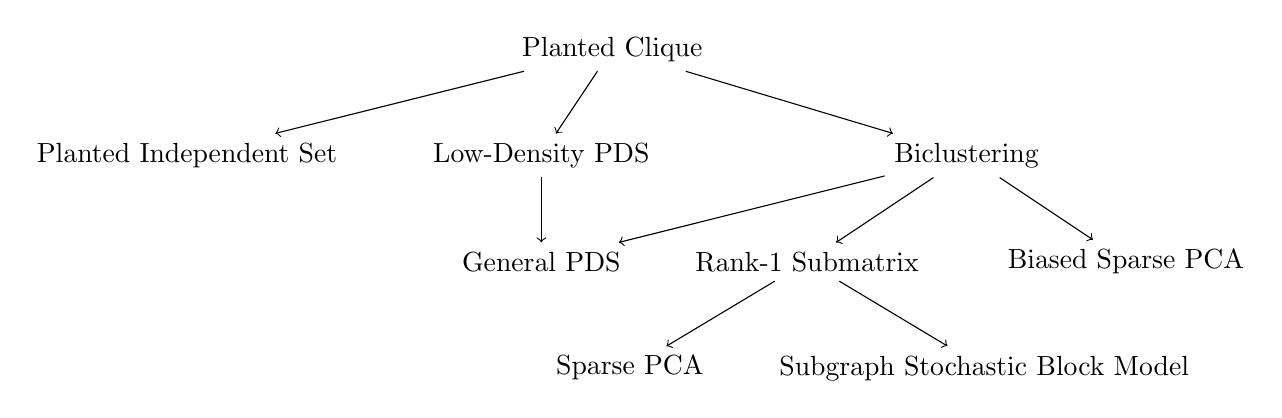
\begin{tikzpicture}[scale=0.45]
\node at (0, 0) (PC) {Planted Clique};
\node at (-12, -3) (PIS) {Planted Independent Set};
\node at (-2, -3) (SPDS) {Low-Density PDS};
\node at (10, -3) (BC) {Biclustering};
\node at (-2, -6) (PDS) {General PDS};
\node at (5.5, -6) (ROS) {Rank-1 Submatrix};
\node at (14.5, -6) (BSPCA) {Biased Sparse PCA};
\node at (0.5, -9) (SPCA) {Sparse PCA};
\node at (10.5, -9) (SSBM) {Subgraph Stochastic Block Model};

\draw[->] (PC) -- (PIS);
\draw[->] (PC) -- (SPDS);
\draw[->] (PC) -- (BC);
\draw[->] (SPDS) -- (PDS);
\draw[->] (BC) -- (PDS);
\draw[->] (BC) -- (BSPCA);
\draw[->] (BC) -- (ROS);
\draw[->] (ROS) -- (SPCA);
\draw[->] (ROS) -- (SSBM);
\end{tikzpicture}
\caption{Graph of average-case reductions for detection problems showing tight statistical-computational gaps given the planted clique conjecture.}
\label{fig:web}
\end{figure*}

The aim of this paper is threefold: (1) to demonstrate that a web of average-case reductions among problems with statistical-computational gaps is feasible even for showing strong computational lower bounds; (2) to introduce a number of new techniques for average-case reductions between problems; and (3) to fully characterize the computationally hard regime of several models. The graph of our reductions is shown in Figure \ref{fig:web}. Our new lower bounds are as follows.
\begin{itemize}
\item \textbf{Planted Independent Set:} We show tight lower bounds for detecting a planted independent set of size $k$ in a sparse Erd\H{o}s-R\'{e}nyi graph of size $n$ with edge density $\tilde{\Theta}(n^{-\alpha})$.
\item \textbf{Planted Dense Subgraph:} If $p > q$ are the edge densities inside and outside of the community, we show the first lower bounds for the general regime $q = \tilde{\Theta}(n^{-\alpha})$ and $p - q = \tilde{\Theta}(n^{-\gamma})$ where $\gamma \ge \alpha$, matching the lower bounds predicted in \cite{chen2016statistical}. Our lower bounds apply to a deterministic community size $k$, resolving a question raised in \cite{hajek2015computational}.
\item \textbf{Biclustering:} We show lower bounds for Gaussian biclustering as a simple hypothesis testing problem to detect a uniformly at random planted flat $k \times k$ submatrix. Our alternative reduction matches the barriers in \cite{ma2015computational}, where a computational lower bound was shown for a composite hypothesis testing variant of biclustering. We show hardness for the natural simple hypothesis testing problem where the $k \times k$ submatrix is chosen uniformly at random and has equal entries.
\item \textbf{Sparse Rank-1 Submatrix:} We show that detection in the sparse spiked Wigner model has a different computational threshold from biclustering when $k \gg \sqrt{n}$. Surprisingly, we are able to obtain tight lower bounds matching these different detection thresholds with different reductions from planted clique.
\item \textbf{Sparse PCA:} We give a reduction between rank-1 submatrix and sparse PCA to obtain tight lower bounds in the less sparse regime $k \gg \sqrt{n}$, when the spectral algorithm is optimal over the SDP. This yields the first tight characterization of a computational barrier for sparse PCA over an entire parameter regime. We also give an alternate reduction recovering the lower bounds of \cite{berthet2013complexity} and \cite{gao2017sparse} in the canonical simple hypothesis testing variant of sparse PCA.
\item \textbf{Biased Sparse PCA:} We show that any assumption on the sparse principal component having a constant fraction more or fewer positive entries than negative entries yields a detection-recovery gap that is not present in sparse PCA. 
\item \textbf{Subgraph Stochastic Block Model:} We introduce a model where two small communities are planted in an Erd\H{o}s-R\'{e}nyi graph of the same average edge density. Parallel to the difference between biclustering and sparse rank-1 submatrix when $k \gg \sqrt{n}$, we show that detection in this model is much harder than in planted dense subgraph when $k \gg \sqrt{n}$.
\end{itemize}
Our lower bounds for planted independent set, the general regime of planted dense subgraph, rank-1 submatrix, sparse PCA when $k \gg \sqrt{n}$, biased sparse PCA and the subgraph stochastic block model are novel. As previously mentioned, lower bounds for sparse PCA when $k \ll \sqrt{n}$, for biclustering and for planted dense subgraph in the sparsest regime were previously known. In each of these cases, we strengthen the existing lower bounds to the apply to the canonical generative model. We show computational lower bounds for simple vs. simple hypothesis testing in all cases other than for sparse PCA, rank-1 submatrix and the subgraph stochastic block model all in the regime $k \gg \sqrt{n}$. This is a consequence of our underlying reduction technique, reflection cloning, and appears unavoidable given our methods. However, we do show that the distribution we reduce to is in some sense close to the canonical generative model.

%Our results demonstrate that, despite the delicate nature of average-case reductions, using natural problems as intermediates can often be beneficial as in reductions in worst-case complexity. Our main technical contribution is to introduce several techniques for mapping problems approximately in total variation without degrading the underlying planted sparse structure. These techniques are:
%\begin{itemize}
%\item \textbf{Distributional Lifting:} A variant of graph lifts that iteratively maps to intermediate matrices with entries from chosen distributions. Varying the underlying distribution produces different relationships between the resulting edge density and size of a planted subgraph. This is in introduced in Sections~\ref{s:lifting}, \ref{s:pds} and~\ref{s:rotations}.
%\item \textbf{Rejection Kernels:} A general framework for a change in measure of the underlying noise distribution while preserving the planted sparse structure. This unifies ideas introduced in \cite{hajek2015computational}, \cite{ma2015computational} and \cite{gao2017sparse}. This is introduced in Section~\ref{s:pds}.
%\item \textbf{Reflection Cloning:} A method of increasing the sparsity of a planted rank-1 structure in noise while preserving the level of signal in the planted structure. This is introduced in Section~\ref{s:reflection}.
%\item \textbf{Random Rotations for Sparse PCA:} An average-case connection between the sparse spiked Wigner model and the spiked covariance model of sparse PCA. This is introduced in Section~\ref{s:rotations}.
%\end{itemize}
%We consider two main variants of distributional lifting using matrices with Poisson and Gaussian entries as intermediates. Poisson and Gaussian lifting lead to two very different parameter scalings, which when combined fully characterize general planted dense subgraph. Reflection cloning can be viewed as a more randomness-efficient variant of Gaussian lifting that we use to show sharper lower bounds for the sparse spiked Wigner model and sparse PCA. We also give algorithms matching our lower bounds and identify the information-theoretic limits of the problems that we consider in Section~\ref{s:info}.

%Although the problems we consider and reduce from planted clique are similar in the sense that they can all be viewed as matrix problems with planted sparse structure, providing tight reductions in total variation that exactly preserve the conjectured computational boundaries proves to be a difficult task and is the main novelty of the present work. A simple example demonstrating this difficulty is our reduction from planted clique to planted independent set. Consider the following naive candidate reduction. Add edges independently to planted clique and then take the complement graph. This maps planted clique to a valid instance of planted independent set with the correct sparse edge density. However, the size of the planted independent set in this proposed reduction turns out to be far smaller than the best known polynomial time algorithms can detect, leaving a gap between the demonstrated and conjectured computational lower bounds. Another example of this lies in the difference between our reductions to biclustering and sparse rank-1 subamtrix. Biclustering is a specific instance of sparse rank-1 submatrix. The reduction we give for biclustering detection is based on a Gaussian variant of distributional lifting and shows tight lower bounds for biclustering. However, this biclustering lower bound turns out to be far below the conjectured lower bound for sparse rank-1 submatrix. We show that a different technique we introduce -- reflection cloning -- that does not apply for biclustering exactly reduces to this stronger lower bound.

\section{Problem Formulations}

\subsection{Detection and Recovery Problems}

We consider problems $\mP$ with planted sparse structure as both detection and recovery tasks, which we denote by $\mP_D$ and $\mP_R$, respectively.

\paragraph{Detection.} In detection problems $\mP_D$, the algorithm is given a set of observations and tasked with distinguishing between two hypotheses:
\begin{itemize}
\item a \emph{uniform} hypothesis $H_0$, under which observations are generated from the natural noise distribution for the problem; and
\item a \emph{planted} hypothesis $H_1$, under which observations are generated from the same noise distribution with a latent planted sparse structure.
\end{itemize}
In all of the detection problems we consider, $H_0$ is a simple hypothesis consisting of a single distribution and $H_1$ is either also simple or a composite hypothesis consisting of several distributions. When $H_1$ is a composite hypothesis, it consists of a set of distributions of the form $P_\theta$ where $\theta$ is the latent sparse structure of interest. Often $H_1$ is a simple hypothesis consisting of a single distribution which is a mixture of $P_\theta$ with $\theta$ in some sense chosen uniformly at random. In both cases, we will abuse notation and refer to $H_1$ as a set of distributions. Given an observation $X$, an algorithm $A(X) \in \{0, 1\}$ \emph{solves} the detection problem \emph{with nontrivial probability} if there is an $\epsilon > 0$ such that its Type I$+$II error satisfies that
$$\limsup_{n \to \infty} \left( \bP_{H_0}[A(X) = 1] + \sup_{\bP \in H_1} \bP_{X \sim \bP}[A(X) = 0] \right) \le 1 - \epsilon$$
where $n$ is the parameter indicating the size of $X$. We refer to this quantity as the asymptotic Type I$+$II error of $A$ for the problem $\mP_D$. If the asymptotic Type I$+$II error of $A$ is zero, then we say $A$ \emph{solves} the detection problem $\mP_D$. Our reductions under total variation all yield exact correspondences between asymptotic Type I$+$II errors. Specifically, they show that if a polynomial time algorithm has asymptotic Type I$+$II error of $\epsilon$ on the problem of interest then there is a polynomial time algorithm with asymptotic Type I$+$II error $\epsilon$ on the problem being reduced from.

\paragraph{Recovery.} In recovery problems $\mP_R$, the algorithm is given an observation from $P_\theta$ for some latent $\theta$ from a space $\Theta$ and the task is to recover the support $S(\theta)$ of the sparse structure $\theta$. There are several variants of the recovery task. Given a randomized algorithm with output $A(X) \in \{ S(\theta) : \theta \in \Theta \}$ and a distribution $\pi$ on the latent space $\Theta$, the variants of the recovery task are as follows.
\begin{itemize}
\item \textit{Partial Recovery}: $A$ solves partial recovery if
$$\bE_{X \sim \bE_\pi P_\theta}[|A(X) \cap S(\theta)|] = \Omega(|S(\theta)|) \quad \text{as } n \to \infty$$
\item \textit{Weak Recovery}: $A$ solves weak recovery if
$$\bE_{X \sim \bE_\pi P_\theta}[|A(X) \Delta S(\theta)|] = o(|S(\theta)|) \quad \text{as } n \to \infty$$
\item \textit{Exact Recovery}: $A$ solves exact recovery with nontrivial probability $\epsilon > 0$ if for all $\theta \in \Theta$
$$\liminf_{n \to \infty} \bP_{X \sim \bE_\pi P_\theta} \left[ A(X) = S(\theta) \right] \ge \epsilon$$
\end{itemize}
Here, $\bE_\pi P_\theta$ denotes the mixture of $P_\theta$ induced by $\pi$ and $\Delta$ denotes the symmetric difference between two sets. Whenever the corresponding detection problem $\mP_D$ has a simple hypothesis $H_1$, $\pi$ will be the prior on $\Theta$ as in $H_1$, which typically is a uniform prior. When $\mP_D$ has a composite hypothesis $H_1$, then an algorithm $A$ solves each of the three variants of the recovery task if the above conditions are met for \emph{all} distributions $\pi$.
%We remark that this is equivalent to the above conditions being met only for distributions $\pi$ with all of their mass on a single $\theta \in \Theta$.
Given a problem $\mP$, the notation $\mP_R$ will denote the exact recovery problem, and $\mP_{PR}$ and $\mP_{WR}$ will denote partial and weak recovery, respectively. All of our recovery reductions will apply to all recovery variants simultaneously.
%In other words, a partial, weak or exact recovery algorithm for the problem of interest implies the same for the problem being reduced from. The computational and statistical barriers for partial, weak and exact recovery generally differ by sub-polynomial factors for the problems we consider. Therefore the polynomial order of the barriers for $\mP_R$ will in general also be those for $\mP_{PR}$ and $\mP_{WR}$. This is discussed in more detail in Section~\ref{s:detectionrecovery}.

%An instance of a detection problem $\mP_D$ hereby refers to an observation $X$. If $\mP_D$ is a simple vs. simple hypothesis testing problem, then the instance $X$ takes one of two distributions -- its distribution under $H_0$ and $H_1$, which we respectively denote by $\mL_{H_0}(X)$ and $\mL_{H_1}(X)$. If $H_1$ is composite, then the distribution of $X$ under $\bP$ is denoted as $\mL_{\bP}(X)$ for each $\bP \in H_1$. An instance of a recovery problem $\mP_R$ refers to an observation from some $P_\theta$ for some latent $\theta \in \Theta$ if the corresponding detection problem has a composite $H_1$ or from $\mL_{H_1}(X) = \bE_\pi P_\theta$ if the corresponding detection problem has a simple $H_1$.

\paragraph{Computational Model.} The algorithms we consider here are either unconstrained or run in randomized polynomial time. An unconstrained algorithm refers to any randomized function or Markov transition kernel from one space to another. These algorithms considered in order to show that information-theoretic lower bounds are asymptotically tight. An algorithm that runs in randomized polynomial time has access to $\text{poly}(n)$ independent random bits and must run in $\text{poly}(n)$ time where $n$ is the size of the input. For clarity of exposition, we assume that explicit expressions can be exactly computed and that $N(0, 1)$ and Poisson random variables can be sampled in $O(1)$ time. %While these assumptions ease the presentation of our reductions, they are unnecessary. The total variation guarantees of our reductions are generally robust to small numerical errors in computing expressions and to total variation errors in sampling distributions. Note that continuous distributions such as $N(0, 1)$ cannot be sampled within total variation less than $1$ with finitely many bits. This issue can rectified by instead considering finite-bit representation variants of problems with continuous data such as sparse PCA, biclustering and rank-1 submatrix. Our reduction methods can be shown to still apply to these discretized models. The details of these discretized reductions and reductions robust to numerical imprecision are in a forthcoming version of the present work.

\subsection{Problems}
\label{ss:formulations}

In this section, we define the problems that we show computational lower bounds for and the conjectures on which these lower bounds are based. Each problem we consider has a natural parameter $n$, which typically denotes the number of samples or dimension of the data, and sparsity parameter $k$. Every parameter for each problem is implicitly a function of $n$, that grows or decays polynomially in $n$. For example, $k = k(n) = \tilde{\Theta}(n^{\beta})$ for some constant $\beta \in (0, 1)$ throughout the paper. For simplicity of notation, we do not write this dependence on $n$. We mostly will be concerned with the polynomial order of growth of each of the parameters and not with subpolynomial factors. We now formally define the problems we consider.

\paragraph{Planted Clique and Independent Set.} The hypotheses in the planted clique detection problem $\textsc{PC}_D(n, k, p)$ are
$$H_0: G \sim G(n, p) \quad \text{and} \quad H_1 : G \sim G(n, k, p)$$
where $G(n, p)$ is an Erd\H{o}s-R\'{e}nyi random graph with edge probability and $G(n, k, p)$ is a sample of $G(n, p)$ with a clique of size $k$ planted uniformly at random. All known polynomial time algorithms for planted clique fail if $k \ll \sqrt{n}$. This has led to the following hardness conjecture.

\begin{conjecture}[PC Conjecture]
Fix some constant $p \in (0, 1)$. Suppose that $\{ A_n \}$ is a sequence of randomized polynomial time algorithms $A_n : \mG_n \to \{0, 1\}$ and $k_n$ is a sequence of positive integers satisfying that $\limsup_{n \to \infty} \log_n k_n < \frac{1}{2}$. Then if $G$ is an instance of $\textsc{PC}_D(n, k, p)$, it holds that
$$\liminf_{n \to \infty} \left( \bP_{H_0}\left[A_n(G) = 1\right] + \bP_{H_1}\left[A_n(G) = 0\right] \right) \ge 1.$$ 
\end{conjecture}

The hardness assumption we use throughout our results is the planted clique conjecture. Other than to show hardness for planted dense subgraph in the sparsest regime, we will only need the planted clique conjecture with edge density $p = 1/2$. An interesting open problem posed in \cite{hajek2015computational} is to show that the PC conjecture at $p = 1/2$ implies it for any fixed constant $p < 1/2$.

The hypotheses in the planted independent set detection problem $\textsc{PIS}_D(n, k, p)$ are
$$H_0: G \sim G(n, p) \quad \text{and} \quad H_1 : G \sim G_I(n, k, p)$$
where $G_I(n, k, p)$ is a sample of $G(n, p)$ where all of the edges of vertex set of size $k$ removed uniformly at random. The recovery $\textsc{PC}_R(n, k, p)$ and $\textsc{PIS}_R(n, k, p)$ problems are to estimate the latent clique and independent set supports given samples from $G(n, k, p)$ and $G_I(n, k, p)$, respectively.

\paragraph{Planted Dense Subgraph.} The hypotheses in the detection problem $\textsc{PDS}_D(n, k, p, q)$ are
$$H_0: G \sim G(n, q) \quad \text{and} \quad H_1 : G \sim G(n, k, p, q)$$
where $G(n, k, p, q)$ is the distribution on $\mG_n$ formed by selecting a size $k$ subset $S$ of $[n]$ uniformly at random and joining every two nodes in $S$ with probability $p$ and every other two nodes with probability $q$. The recovery problem $\textsc{PDS}_R(n, k, p, q)$ is to estimate the latent planted dense subgraph support $S$ given samples from $G(n, k, p, q)$.

A phenomenon observed in \cite{hajek2015computational} and in \cite{chen2016statistical} is that planted dense subgraph appears to have a detection-recovery gap in the regime where $k \gg \sqrt{n}$. The following is a formulation of the conjectured sharper recovery lower bound.

\begin{conjecture}[PDS Recovery Conjecture] Suppose that $G \sim G(n, k, p, q)$ and
$$\liminf_{n \to \infty} \log_n k > \frac{1}{2} \quad \text{and} \quad \limsup_{n \to \infty} \log_n \left(\frac{k^2(p-q)^2}{q(1-q)} \right) < 1$$
then there is no sequence of randomized polynomial-time algorithms $A_n : \mG_n \to \binom{[n]}{k}$ such that $A_n(G)$ achieve exact recovery of the vertices in the latent planted dense subgraph as $n \to \infty$.
\end{conjecture}

This conjecture asserts that the threshold of $n/k^2$ on the signal $\frac{(p-q)^2}{q(1 - q)}$ of an instance of PDS is tight for the recovery problem. In contrast, our results show that the tight detection threshold for PDS given the PC conjecture is lower, at $n^2/k^4$. We will use this conjecture to establish similar detection-recovery gaps for biased sparse PCA and biclustering. We note that a related detection-recovery gap for BC was shown in \cite{cai2015computational}. The same lower bound was established for strong recovery algorithms that solve biclustering for all subgaussian noise distributions assuming hardness of planted clique for a different distribution on random graphs than Erd\H{o}s-R\'{e}nyi.

\paragraph{Subgraph Stochastic Block Model.} We introduce a planted subgraph variant of the two community stochastic block model without the edge-thresholding test that produced the conjectural detection-recovery gap in planted dense subgraph. Let $G_B(n, k, q, \rho)$ denote the set of distributions on $\mG_n$ generated a graph $G$ as follows. Fix any two positive integers $k_1$ and $k_2$ satisfying that
$$\frac{k}{2} - k^{1-\delta} \le k_1, k_2 \le \frac{k}{2} + k^{1 - \delta}$$
where $\delta = \delta_{\text{SSBM}} > 0$ is a small constant that will remained fixed throughout the paper. Let $S = [k_1]$ and $T = [k_1+k_2]\backslash [k_1]$. Then generate the edges of $G$ independently as follows:
\begin{enumerate}
\item include edges within $S$ or within $T$ with probability at least $q + \rho$;
\item include edges between $S$ and $T$ with probability at most $q - \rho$; and
\item include all other edges with probability $q$.
\end{enumerate}
Then permute the vertices of $G$ according to a permutation selected uniformly at random. The communities of the graph are defined to be the images of $S$ and $T$ under this permutation. Note that $G_B(n, k, q, \rho)$ defines a set of distributions since $k_1$ and $k_2$ are permitted to vary and the edges between $S$ and $T$ are included independently with a probability at least $q + \rho$ for each edge. Thus given the random permutation, $G$ is distributed as an inhomogeneous random graph with independent edges. The subgraph stochastic block model detection problem $\textsc{SSBM}_D(n, k, q, \rho)$ has hypotheses given by
$$H_0: G \sim G(n, q) \quad \text{and} \quad H_1 : G \sim \bP \quad \text{ for some } \quad \bP \in G_B(n, k, q, \rho)$$

\paragraph{Biclustering.} Let $\mathcal{M}_{n, k} \subseteq \mathbb{R}^{n \times n}$ be the set of sparse matrices supported on a $k \times k$ submatrix with each nonzero entry equal to $1$. The biclustering detection problem $\textsc{BC}_D(n, k, \mu)$ has hypotheses
$$H_0: M \sim N(0, 1)^{\otimes n \times n} \quad \text{and} \quad H_1 : M \sim \mu \cdot A + N(0, 1)^{\otimes n \times n} \text{ where } A \sim \text{Unif}\left[\mathcal{M}_{n,k}\right]$$
The recovery problem $\textsc{BC}_R$ is to estimate the latent support matrix $A$ given a sample from $H_1$.

\paragraph{Rank-1 Submatrix and Sparse Spiked Wigner.} In rank-1 submatrix, sparse spiked Wigner and sparse PCA, the planted sparse vectors will have sufficiently large entries for support recovery to be possible. We consider the following set of near-uniform magnitude unit vectors
$$\mathcal{V}_{d,k} = \left\{ v \in \mathbb{S}^{d-1}  : k - \frac{k}{\log k} \le \| v \|_0 \le k \text{ and } |v_i| \ge \frac{1}{\sqrt{k}} \text{ for } i \in \text{supp}(v) \right\}$$
The function $\log k$ can be replaced by any sub-polynomially growing function but is given explicitly for simplicity. The detection problem $\textsc{ROS}_D(n, k, \mu)$ has hypotheses
$$H_0: M \sim N(0, 1)^{\otimes n \times n} \quad \text{and} \quad H_1 : M \sim \mu \cdot rc^\top + N(0, 1)^{\otimes n \times n} \text{ where } r, c \in \mathcal{V}_{n, k}$$
The recovery problem $\textsc{ROS}_R$ is to estimate the latent supports $\text{supp}(r)$ and $\text{supp}(c)$. An $n \times n$ GOE matrix $\text{GOE}(n)$ is a symmetric matrix with i.i.d. $N(0, 1)$ entries below its main diagonal and i.i.d. $N(0, 2)$ entries on its main diagonal. The sparse spiked Wigner detection problem $\textsc{SSW}_D$ has hypotheses
$$H_0: M \sim \text{GOE}(n) \quad \text{and} \quad H_1 : M \sim \mu \cdot rr^\top + \text{GOE}(n) \text{ where } r \in \mathcal{V}_{n, k}$$
and the recovery problem $\textsc{SSW}_R$ is to estimate the latent supports $\text{supp}(r)$. A simple intermediate variant that will be useful in our reductions is $\textsc{SROS}$, which is $\textsc{ROS}$ constrained to have a symmetric spike $r = c$. Note that if $M$ is an instance of $\textsc{SROS}_D(n, k, \mu)$ then it follows that $\frac{1}{\sqrt{2}}(M + M^\top)$ is an instance of $\textsc{SSW}_D(n, k, \mu/\sqrt{2})$.

\paragraph{Sparse PCA.} Detection in the \emph{spiked covariance model} of $\textsc{SPCA}_D(n, k, d, \theta)$ has hypotheses
\begin{align*}
&H_0: X_1, X_2, \dots, X_n \sim N(0, I_d)^{\otimes n} \quad \text{and} \\
&H_1 : X_1, X_2, \dots, X_n \sim N\left(0, I_d + \theta vv^\top\right)^{\otimes n} \text{ where } v \in \mathcal{V}_{d, k}
\end{align*}
The recovery task $\textsc{SPCA}_R$ is to estimate $\text{supp}(v)$ given observations $X_1, X_2, \dots, X_n$ sampled from $N\left(0, I_d + \theta vv^\top\right)^{\otimes n}$ where $v \in \mathcal{V}_{d, k}$. We also consider a simple hypothesis testing variant $\textsc{USPCA}_D$ of sparse PCA with a simple hypothesis $H_1$ where $v$ is chosen uniformly at random from the set $S_k \subseteq \mathbb{R}^d$ of all $k$-sparse unit vectors with nonzero coordinates equal to $\pm 1/\sqrt{k}$.

\paragraph{Biased Sparse PCA.} We introduce a variant of the spiked covariance model with an additional promise. In particular, $v$ is restricted to the set $\mathcal{BV}_{d, k}$ of vectors in $\mathcal{V}_{d,k}$ with some overall positive or negative bias. Formally, if $\| v \|_0^+$ denotes the number of positive entries of $v$ then
$$\mathcal{BV}_{d, k} = \left\{ v \in \mathcal{V}_{d, k} : \| v \|_0^+ \ge \left( \frac{1}{2} + \delta \right) k \text{ or } \| v \|_0^+ \le \left( \frac{1}{2} - \delta \right) k \right\}$$
where $\delta = \delta_{\textsc{BSPCA}} > 0$ is an arbitrary constant that will remain fixed throughout the paper. The detection problem $\textsc{BSPCA}_D(n, k, d, \theta)$ has the same hypotheses as $\textsc{SPCA}_D(n, k, d, \theta)$ with the added constraint $v \in \mathcal{BV}_{d, k}$. The recovery problem $\textsc{BSPCA}_R$ is do estimate $\text{supp}(v)$ given observations $X_1, X_2, \dots, X_n$ sampled from $N\left(0, I_d + \theta vv^\top\right)^{\otimes n}$ where $v \in \mathcal{BV}_{d, k}$. We also consider a simple hypothesis testing variant $\textsc{UBSPCA}_D$ defined similarly to $\textsc{USPCA}_D$ with $v \sim \text{Unif}[BS_k]$ where $BS_k$ is the set of all $k$-sparse unit vectors with nonzero coordinates equal to $1/\sqrt{k}$.

\section{Summary of Results}

%In this paper, our aim is to establish tight characterizations of the statistical-computational gaps for the problems formulated in the previous section.
Each problem has three regimes for each of its detection and recovery variants. In the easy regime, there is a polynomial-time algorithm for the task. In the hard regime, the PC or PDS recovery conjecture implies that there is no polynomial-time algorithm but there is an inefficient algorithm solving the task. In the impossible regime, the task is information-theoretically impossible.
%Our results complete the hardness picture for each of these problems other than sparse PCA when $k \ll \sqrt{n}$ and biased sparse PCA.
Our results are informally stated below and depicted visually in Figure \ref{fig:diagrams} in Appendix \ref{sec:figmain}.

\begin{theorem}[Informal Main Theorem] \label{lem:2a}
Given the PC and PDS recovery conjectures, the easy, hard and impossible regimes of the problems in Section~\ref{ss:formulations} are classified in Figure~\ref{fig:classification} as following one of the configurations of regimes in Figure~\ref{fig:types}.
%\begin{enumerate}
%\item $\textsc{PIS}_D(n, k, q)$ and $\textsc{PDS}_D(n, k, cq, q)$ in the regime $q = \tilde{\Theta}(n^{-\alpha})$ for some fixed $\alpha \in [0, 1)$ and constant $c > 1$, has regions
%\begin{align*}
%&\bullet \, \, \mathbf{Easy} \left\{ \begin{array}{ll} q \gtrsim \frac{n^2}{k^4} &\text{if } k \gtrsim \sqrt{n} \end{array} \right. \quad \quad  \bullet \, \, \mathbf{Hard} \left\{ \begin{array}{ll} q \gtrsim \frac{1}{k} &\text{if } k \ll \sqrt{n} \\ \frac{n^2}{k^4} \gg q \gtrsim \frac{1}{k} &\text{if } \sqrt{n} \lesssim k \ll n^{2/3} \end{array} \right. \\
%& \bullet \, \, \mathbf{Impossible} \left\{ \begin{array}{ll} q \ll \frac{1}{k} &\text{if } k \ll n^{2/3} \\ q \ll \frac{n^2}{k^4} &\text{if } k \gtrsim n^{2/3} \end{array} \right.
%\end{align*}
%\item $\textsc{PIS}_R(n, k, q)$ and $\textsc{PDS}_R(n, k, cq, q)$ in the regime $q = \tilde{\Theta}(n^{-\alpha})$ for some fixed $\alpha \in [0, 1)$ and constant $c > 1$, has regions
%\begin{align*}
%&\bullet \, \, \mathbf{Easy} \left\{ \begin{array}{ll} q \gtrsim \frac{n}{k^2} &\text{if } k \gtrsim \sqrt{n} \end{array} \right. \quad \quad  \bullet \, \, \mathbf{Hard} \left\{ \begin{array}{ll} q \gtrsim \frac{1}{k} &\text{if } k \ll \sqrt{n} \\ \frac{n}{k^2} \gg q \gtrsim \frac{1}{k} &\text{if } \sqrt{n} \lesssim k \ll n^{2/3} \end{array} \right. \\
%& \bullet \, \, \mathbf{Impossible} \left\{ \begin{array}{ll} q \ll \frac{1}{k} \end{array} \right.
%\end{align*}
%\item $\textsc{PDS}_D(n, k, p, q)$ in the regime $p > q$, $q = \tilde{\Theta}(n^{-\alpha})$ and $p - q = \tilde{\Theta}(n^{-\gamma})$ for some fixed $\alpha, \gamma \in [0, 1)$ with $\gamma \ge \alpha$, has regions
%\begin{align*}
%&\bullet \, \, \mathbf{Easy} \left\{ \begin{array}{ll} \frac{(p - q)^2}{q(1 -q)} \gtrsim \frac{n^2}{k^4} &\text{if } k \gtrsim \sqrt{n} \end{array} \right. \quad \quad  \bullet \, \, \mathbf{Hard} \left\{ \begin{array}{ll} \frac{(p - q)^2}{q(1 -q)} \gtrsim \frac{1}{k} &\text{if } k \ll \sqrt{n} \\ \frac{n^2}{k^4} \gg \frac{(p - q)^2}{q(1 -q)} \gtrsim \frac{1}{k} &\text{if } \sqrt{n} \lesssim k \ll n^{2/3} \end{array} \right. \\
%& \bullet \, \, \mathbf{Impossible} \left\{ \begin{array}{ll} \frac{(p - q)^2}{q(1 -q)} \ll \frac{1}{k} &\text{if } k \ll n^{2/3} \\ \frac{(p - q)^2}{q(1 -q)} \ll \frac{n^2}{k^4} &\text{if } k \gtrsim n^{2/3} \end{array} \right.
%\end{align*}
%\item$\textsc{PDS}_R(n, k, p, q)$ in the regime $p > q$, $q = \tilde{\Theta}(n^{-\alpha})$ and $p - q = \tilde{\Theta}(n^{-\gamma})$ for some fixed $\alpha, \gamma \in [0, 1)$ with $\gamma \ge \alpha$, has regions
%\begin{align*}
%&\bullet \, \, \mathbf{Easy} \left\{ \begin{array}{ll} \frac{(p - q)^2}{q(1 -q)} \gtrsim \frac{n}{k^2} &\text{if } k \gtrsim \sqrt{n} \end{array} \right. \quad \quad  \bullet \, \, \mathbf{Hard} \left\{ \begin{array}{ll} \frac{(p - q)^2}{q(1 -q)} \gtrsim \frac{1}{k} &\text{if } k \ll \sqrt{n} \\ \frac{n}{k^2} \gg \frac{(p - q)^2}{q(1 -q)} \gtrsim \frac{1}{k} &\text{if } \sqrt{n} \lesssim k \end{array} \right. \\
%& \bullet \, \, \mathbf{Impossible} \left\{ \begin{array}{ll} \frac{(p - q)^2}{q(1 -q)} \ll \frac{1}{k} \end{array} \right.
%\end{align*}
%\item $\textsc{PSBM}_D(n, k, q, \rho)$ and $\textsc{PSBM}_R(n, k, q, \rho)$ in the regime $q = \theta(1)$ and $\rho = \tilde{\Theta}(n^{-\alpha})$ for some fixed $\alpha \in [0, 1)$, has regions
%\begin{align*}
%&\bullet \, \, \mathbf{Easy} \left\{ \begin{array}{ll} \rho \gtrsim \frac{\sqrt{n}}{k} &\text{if } k \gtrsim \sqrt{n} \end{array} \right. \quad \quad  \bullet \, \, \mathbf{Hard} \left\{ \begin{array}{ll} \rho \gtrsim \frac{1}{\sqrt{k}} &\text{if } k \ll \sqrt{n} \\ \frac{\sqrt{n}}{k} \gg \rho \gtrsim \frac{1}{\sqrt{k}} &\text{if } k \gtrsim \sqrt{n} \end{array} \right. \\
%& \bullet \, \, \mathbf{Impossible} \left\{ \begin{array}{ll} \rho \ll \frac{1}{\sqrt{k}} \end{array} \right.
%\end{align*}
%\item $\textsc{BC}_D(n, k, \mu)$ in the regime $\mu = \tilde{\Theta}(n^{-\alpha})$ for some fixed $\alpha \in [0, 1)$, has regions
%\begin{align*}
%&\bullet \, \, \mathbf{Easy} \left\{ \begin{array}{ll} \mu \gtrsim 1 &\text{if } k \ll \sqrt{n} \\ \mu \gtrsim \frac{n}{k^2} &\text{if } k \gtrsim \sqrt{n} \end{array} \right. \quad \quad  \bullet \, \, \mathbf{Hard} \left\{ \begin{array}{ll} 1 \gg \mu \gtrsim \frac{1}{\sqrt{k}} &\text{if } k \ll \sqrt{n} \\ \frac{n}{k^2} \gg \mu \gtrsim \frac{1}{\sqrt{k}} &\text{if } \sqrt{n} \lesssim k \ll n^{2/3} \end{array} \right. \\
%& \bullet \, \, \mathbf{Impossible} \left\{ \begin{array}{ll} \mu \ll \frac{1}{\sqrt{k}} &\text{if } k \ll n^{2/3} \\ \mu \ll \frac{n}{k^2} &\text{if } k \gtrsim n^{2/3} \end{array} \right.
%\end{align*}
%\item $\textsc{BC}_R(n, k, \mu)$ in the regime $\mu = \tilde{\Theta}(n^{-\alpha})$ for some fixed $\alpha \in [0, 1)$, has regions
%\begin{align*}
%&\bullet \, \, \mathbf{Easy} \left\{ \begin{array}{ll} \mu \gtrsim 1 &\text{if } k \ll \sqrt{n} \\ \mu \gtrsim \frac{\sqrt{n}}{k} &\text{if } k \gtrsim \sqrt{n} \end{array} \right. \quad \quad  \bullet \, \, \mathbf{Hard} \left\{ \begin{array}{ll} 1 \gg \mu \gtrsim \frac{1}{\sqrt{k}} &\text{if } k \ll \sqrt{n} \\ \frac{\sqrt{n}}{k} \gg \mu \gtrsim \frac{1}{\sqrt{k}} &\text{if } k \gtrsim \sqrt{n} \end{array} \right. \\
%& \bullet \, \, \mathbf{Impossible} \left\{ \begin{array}{ll} \mu \ll \frac{1}{\sqrt{k}} \end{array} \right.
%\end{align*}
%\item $\textsc{ROS}_D(n, k, \mu)$ and $\textsc{ROS}_R(n, k, \mu)$ in the regime $\mu = \tilde{\Theta}(n^{-\alpha})$ for some fixed $\alpha \in [0, 1)$, have regions
%\begin{align*}
%&\bullet \, \, \mathbf{Easy} \left\{ \begin{array}{ll} \mu \gtrsim k &\text{if } k \ll \sqrt{n} \\ \mu \gtrsim \sqrt{n} &\text{if } k \gtrsim \sqrt{n} \end{array} \right. \quad \quad  \bullet \, \, \mathbf{Hard} \left\{ \begin{array}{ll} k \gg \mu \gtrsim \sqrt{k} &\text{if } k \ll \sqrt{n} \\ \sqrt{n} \gg \mu \gtrsim \sqrt{k} &\text{if } k \gtrsim \sqrt{n} \end{array} \right. \\
%& \bullet \, \, \mathbf{Impossible} \left\{ \begin{array}{ll} \mu \ll \sqrt{k} \end{array} \right.
%\end{align*}
%\item $\textsc{SPCA}_D(n, k, d, \theta)$, $\textsc{SPCA}_R(n, k, d, \theta)$ and $\textsc{BSPCA}_R(n, k, d, \theta)$ in the regime $d = \Theta(n)$ and $\theta = \tilde{\Theta}(n^{-\alpha})$ for some $\alpha \in [0, 1)$, have regions
%\begin{align*}
%&\bullet \, \, \mathbf{Easy} \left\{ \begin{array}{ll} \theta \gtrsim \frac{k}{\sqrt{n}} &\text{if } k \ll \sqrt{n} \\ \theta \gtrsim 1 &\text{if } k \gtrsim \sqrt{n} \end{array} \right. \quad \quad  \bullet \, \, \mathbf{Hard} \left\{ \begin{array}{ll} \frac{k^2}{n} \gg \theta \gtrsim \sqrt{\frac{k}{n}} &\text{if } k \ll \sqrt{n} \\ 1 \gg \theta \gtrsim \sqrt{\frac{k}{n}} &\text{if } k \gtrsim \sqrt{n} \end{array} \right. \\
%& \bullet \, \, \mathbf{Impossible} \left\{ \begin{array}{ll} \theta \ll \sqrt{\frac{k}{n}} \end{array} \right.
%\end{align*}
%\item $\textsc{BSPCA}_D(n, k, d, \theta)$ in the regime $d = \Theta(n)$ and $\theta = \tilde{\Theta}(n^{-\alpha})$ for some $\alpha \in [0, 1)$, has regions
%\begin{align*}
%&\bullet \, \, \mathbf{Easy} \left\{ \begin{array}{ll} \theta \gtrsim \frac{k}{\sqrt{n}} &\text{if } k \ll \sqrt{n} \\ \theta \gtrsim \frac{\sqrt{n}}{k} &\text{if } k \gtrsim \sqrt{n} \end{array} \right. \quad \quad  \bullet \, \, \mathbf{Hard} \left\{ \begin{array}{ll} \frac{k^2}{n} \gg \theta \gtrsim \sqrt{\frac{k}{n}} &\text{if } k \ll \sqrt{n} \\ \frac{n}{k^2} \gg \theta \gtrsim \sqrt{\frac{k}{n}} &\text{if } \sqrt{n} \lesssim k \ll n^{2/3} \end{array} \right. \\
%&\bullet \, \, \mathbf{Impossible} \left\{ \begin{array}{ll} \theta \ll \sqrt{\frac{k}{n}} &\text{if } k \ll n^{2/3} \\ \theta \ll \frac{\sqrt{n}}{k} &\text{if } k \gtrsim n^{2/3} \end{array} \right.
%\end{align*}
%\end{enumerate}
\end{theorem}

\begin{figure*}
\begin{center}
\begin{tabular}{|c | c c c|}
\hline
\textsc{Type I} & $k \ll n^{1/2}$ & $n^{1/2} \lesssim k \ll n^{2/3}$ & $n^{2/3} \ll k$ \\
\hline
\textnormal{Impossible} & $\textnormal{SNR} \ll \frac{1}{k}$ & $\textnormal{SNR} \ll \frac{1}{k}$ & $\textnormal{SNR} \ll \frac{n^2}{k^4}$ \\
\textnormal{Hard} & $\textnormal{SNR} \gtrsim \frac{1}{k}$ & $\frac{1}{k} \lesssim \textnormal{SNR} \ll \frac{n^2}{k^4}$ & \textnormal{None} \\
\textnormal{Easy} & (A) \textnormal{None} & $\textnormal{SNR} \gtrsim \frac{n^2}{k^4}$ & $\textnormal{SNR} \gtrsim \frac{n^2}{k^4}$ \\
& (B) $\textnormal{SNR} \gtrsim 1$ & & \\
\hline
\end{tabular}
\vspace{5mm}

\begin{tabular}{|c | c c c|}
\hline
\textsc{Type II} & $k \ll n^{1/2}$ & $n^{1/2} \lesssim k \ll n^{2/3}$ & $n^{2/3} \ll k$ \\
\hline
\textnormal{Impossible} & $\textnormal{SNR} \ll \sqrt{\frac{k}{n}}$ & $\textnormal{SNR} \ll \sqrt{\frac{k}{n}}$ & $\textnormal{SNR} \ll \sqrt{\frac{n}{k^2}}$ \\
\textnormal{Hard} & $\sqrt{\frac{k}{n}} \lesssim \textnormal{SNR} \ll \frac{k^2}{n}$ & $\sqrt{\frac{k}{n}} \lesssim \textnormal{SNR} \ll \frac{n}{k^2}$ & \textnormal{None} \\
\textnormal{Easy} & $\textnormal{SNR} \gtrsim \sqrt{\frac{k^2}{n}}$ & $\textnormal{SNR} \gtrsim \sqrt{\frac{n}{k^2}}$ & $\textnormal{SNR} \gtrsim \sqrt{\frac{n}{k^2}}$ \\
\hline
\end{tabular}
\vspace{5mm}

\resizebox{\textwidth}{!}{
\begin{tabular}{|c | c c | c | c c |}
\hline
\textsc{Type III} & $k \ll n^{1/2}$ & $n^{1/2} \lesssim k$ & \textsc{Type IV} & $k \ll n^{1/2}$ & $n^{1/2} \lesssim k$ \\
\hline
\textnormal{Impossible} & $\textnormal{SNR} \ll \frac{1}{k}$ & $\textnormal{SNR} \ll \frac{1}{k}$ & \textnormal{Impossible} & $\textnormal{SNR} \ll \sqrt{\frac{k}{n}}$ & $\textnormal{SNR} \ll \sqrt{\frac{k}{n}}$ \\
\textnormal{Hard} & $\textnormal{SNR} \gtrsim \frac{1}{k}$ & $\frac{1}{k} \lesssim \textnormal{SNR} \ll \frac{n}{k^2}$ & \textnormal{Hard} & $\sqrt{\frac{k}{n}} \lesssim \textnormal{SNR} \ll \frac{k^2}{n}$ & $\sqrt{\frac{k}{n}} \lesssim \textnormal{SNR} \ll 1$ \\
\textnormal{Easy} & (A) \textnormal{None} & $\textnormal{SNR} \gtrsim \frac{n}{k^2}$ & \textnormal{Easy} & $\textnormal{SNR} \gtrsim \sqrt{\frac{k^2}{n}}$ & $\textnormal{SNR} \gtrsim 1$ \\
& (B) $\textnormal{SNR} \gtrsim 1$ & & & & \\
\hline
\end{tabular}}
\end{center}
\caption{Types of hardness regimes by $\text{SNR}$ in Theorem \ref{lem:2a}. \textsc{Type I} and \textsc{Type III} each have two variants A and B depending on the Easy regime when $k \ll n^{1/2}$.}
\label{fig:types}
\end{figure*}
\begin{figure*}
\begin{center}
\begin{tabular}{| c | c | c | c |}
\hline
\textsc{Problems} & \textsc{Parameter Regime} & \textsc{SNR} & \textsc{Type} \\
\hline
$\textsc{PIS}_D(n, k, q), \textsc{PDS}_D(n, k, cq, q)$ & $q = \tilde{\Theta}(n^{-\alpha})$ for fixed $\alpha \in [0, 1)$ and $c > 1$ & $q$ & \textsc{Type IA} \\
\hline
$\textsc{PIS}_R(n, k, q), \textsc{PDS}_R(n, k, cq, q)$ & $q = \tilde{\Theta}(n^{-\alpha})$ for fixed $\alpha \in [0, 1)$ and $c > 1$ & $q$ & \textsc{Type IIIA} \\
\hline
$\textsc{PDS}_D(n, k, p, q)$ & $q = \tilde{\Theta}(n^{-\alpha})$ and $p - q = \tilde{\Theta}(n^{-\gamma})$ with & $\frac{(p - q)^2}{q(1 - q)}$ & \textsc{Type IA} \\
& $p > q$ for fixed $\alpha, \gamma \in [0, 1)$ & & \\
\hline
$\textsc{PDS}_R(n, k, p, q)$ & $q = \tilde{\Theta}(n^{-\alpha})$ and $p - q = \tilde{\Theta}(n^{-\gamma})$ with & $\frac{(p - q)^2}{q(1 - q)}$ & \textsc{Type IIIA} \\
& $p > q$ for fixed $\alpha, \gamma \in [0, 1)$ & & \\
\hline
$\textsc{SSBM}_D(n, k, q, \rho)$ & $q = \Theta(1)$ and $\rho = \tilde{\Theta}(n^{-\alpha})$ & $\rho^2$ & \textsc{Type IIIA} \\
 & for fixed $\alpha \in [0, 1)$ & & \\
\hline
$\textsc{BC}_D(n, k, \mu)$ & $\mu = \tilde{\Theta}(n^{-\alpha})$ for fixed $\alpha \in [0, 1)$ & $\mu^2$ & \textsc{Type IB} \\
\hline
$\textsc{BC}_R(n, k, \mu)$ & $\mu = \tilde{\Theta}(n^{-\alpha})$ for fixed $\alpha \in [0, 1)$ & $\mu^2$ & \textsc{Type IIIB} \\
\hline
$\textsc{ROS}_D(n, k, \mu)$, $\textsc{ROS}_R(n, k, \mu)$, & $\mu = \tilde{\Theta}(n^{-\alpha})$ for fixed $\alpha \in [0, 1)$ & $\frac{\mu^2}{k^2}$ & \textsc{Type IIIB} \\
$\textsc{SSW}_D(n, k, \mu)$, $\textsc{SSW}_R(n, k, \mu)$ & & & \\
\hline
$\textsc{SPCA}_D(n, k, d, \theta)$, & $d = \Theta(n)$ and $\theta = \tilde{\Theta}(n^{-\alpha})$ & $\theta$ & \textsc{Type II} \\
$\textsc{SPCA}_{WR}(n, k, d, \theta)$, & for fixed $\alpha \in [0, 1)$ & & \\
$\textsc{BSPCA}_{WR}(n, k, d, \theta)$ & & & \\
\hline
$\textsc{BSPCA}_D(n, k, d, \theta)$ & $d = \Theta(n)$ and $\theta = \tilde{\Theta}(n^{-\alpha})$  & $\theta$ & \textsc{Type IV} \\
& for fixed $\alpha \in [0, 1)$ & & \\
\hline
\end{tabular}
\end{center}
\caption{Classification of regimes for each problem as in Theorem \ref{lem:2a}. For each problem, $k$ is in the regime $k = \tilde{\Theta}(n^{\beta})$ where $\beta \in (0, 1)$ is a constant.}
\label{fig:classification}
\end{figure*}

We remark that all of the computational lower bounds in Theorem \ref{lem:2a} follow from the PC conjecture other than those for $\textsc{PIS}_R, \textsc{PDS}_R, \textsc{BC}_R$ and $\textsc{BSPCA}_{WR}$ which follow from the PDS conjecture.
%The computational lower bounds implicit in the hard regimes in Figures~\ref{fig:types} and~\ref{fig:classification} are the focus of the present work.
Appendix~\ref{s:lifting} introduces $\textsc{PC-Lifting}$ to reduce from $\textsc{PC}_D$ to $\textsc{PIS}_D$. Section~\ref{s:rejection} introduces rejection kernels and general $\textsc{Distributional-Lifting}$ which are then applied in Appendix~\ref{s:pds} to reduce from $\textsc{PC}_D$ to all regimes of $\textsc{PDS}_D$. Appendix~\ref{s:reflection} introduces reflection cloning to reduce from $\textsc{BC}_D$ to $\textsc{ROS}_D$, $\textsc{SSW}_D$ and $\textsc{SSBM}_D$. Section~\ref{s:rotations} introduces random rotations to reduce from $\textsc{SSW}_D$ to $\textsc{SPCA}_D$ and from $\textsc{BC}_D$ to $\textsc{BSPCA}_D$. In Appendix~\ref{s:pds}, we also give a reduction from $\textsc{PDS}_R$ to $\textsc{BC}_R$ and in Appendix~\ref{s:rotations}, we reduce from $\textsc{PDS}_R$ to $\textsc{BSPCA}_{WR}$. In Section~\ref{s:info}, we establish the algorithmic upper bounds and information-theoretic lower bounds in Theorem \ref{lem:2a}. In Appendix~\ref{s:detectionrecovery}, we show that our detection lower bounds imply recovery lower bounds. Note that this gives a complete characterization of the easy, hard and impossible regions for all of the problems we consider other than sparse PCA and biased sparse PCA. The SDP relaxation of the MLE for sparse PCA succeeds if $d = \Theta(n)$ and $k \ll \sqrt{n}$ down to the signal level of $\theta \approx k/\sqrt{n}$, which is generally conjectured to be optimal. There is a gap between the lower bounds we prove here, which match those of \cite{berthet2013optimal} and \cite{gao2017sparse} and this conjecturally optimal threshold when $k \ll \sqrt{n}$.
%There is also a gap for biased sparse PCA detection when $k \gg \sqrt{n}$. These gaps are depicted as the black region in Figures \ref{fig:diagrams}(f) and \ref{fig:diagrams}(g). Showing tight hardness for sparse PCA for any parameters $k \ll \sqrt{n}$ remains an interesting open problem. Notably, we do not consider the recovery problem for the subgraph stochastic block model and only consider weak, rather than exact, recovery for sparse PCA and biased sparse PCA. While we obtain computational lower bounds that apply to these recovery variants, obtaining matching information-theoretic lower bounds and algorithms remains an open problem. These open problems are discussed in more detail in Section~\ref{s:future}.
We also do not consider the recovery problem for the subgraph stochastic block model and only consider weak, rather than exact, recovery for sparse PCA and biased sparse PCA.

%In Figure \ref{fig:diagrams} and Theorem \ref{lem:2a}, we depict the implications of our hardness results for $\textsc{SPCA}$ and $\textsc{BSPCA}$ in the case where $d = \Theta(n)$ for simplicity. Our hardness results extend mildly beyond this regime, but not tightly. However, we remark that the assumptions $d = \Theta(n)$ or $d = \Omega(n)$ have become commonplace in the literature on lower bounds for sparse PCA. The reductions from PC to sparse PCA in \cite{berthet2013complexity}, \cite{wang2016statistical} and \cite{gao2017sparse} construct hard instances that are only tight when $d = \Omega(n)$. The sum of squares lower bounds for sparse PCA in \cite{ma2015sum} and \cite{hopkins2017power} also are in the regime $d = \Theta(n)$. The SOS lower bounds in \cite{hopkins2017power} are actually for the spiked Wigner model rather than the spiked covariance model of sparse PCA that we consider.

\section{Techniques}

Our main technical contribution is to introduce four techniques for mapping problems approximately in total variation without degrading the underlying planted sparse structure.

\paragraph{Distributional Lifting.} We introduce several new techniques resembling graph lifts to increase the size $k$ of a sparse structure, while appropriately maintaining the level of signal and independence in the noise distribution. Given a graph $G$, the main idea behind our techniques is to replace the $\{0, 1\}$-valued edge indicators with Gaussian and Poisson random variables. We then increase the size of an instance by a factor of two iteratively, while maintaining the signal and independence, through distributional tricks such as Poisson thinning and the rotational invariance of independent Gaussians. In \cite{hajek2015computational}, the reduction from planted clique to planted dense subgraph also expands an input graph. Rather than proceed iteratively, their method expands the graph in one step. The main technical issue arising from this is that the diagonal entries of the graph's adjacency matrix are mapped to low-density subgraphs in the hidden community. Showing that these are not detectable requires a subtle argument and that the hidden community is randomly sized according to a Binomial distribution. By proceeding incrementally as in our approach, the diagonal entries become much easier to handle. However for many regimes of interest, incremental approaches that preserve the fact that the instance is a graph seem to unavoidably introduce dependence between edges. Our insight is to map edges to other random variables that can be preserved incrementally while maintaining independence and the desired parameter scaling to produce tight lower bounds. Using Poisson and Gaussian variants of this lifting procedure, we are able to reduce from planted clique in a wide range of parameter regimes. Gaussian lifting also recover a simple vs. simple hypothesis testing variant of the lower bounds for biclustering shown in \cite{ma2015computational} as an intermediate step towards reducing to planted dense subgraph.

\paragraph{Rejection Kernels.} We give a simple scheme based on rejection sampling that approximately maps a sample from $\text{Bern}(p)$ to a sample from $P$ and from $\text{Bern}(q)$ to $Q$ where $p, q \in [0, 1]$ and $P$ and $Q$ are two distributions on $\mathbb{R}$. By truncating samples from a pair of distributions $P'$ and $Q'$, and then mapping the resulting Bernoulli random variables to a pair of target distributions $P$ and $Q$, this method yields an efficient procedure to simultaneously perform two changes of measure. This method is used in distributional lifting to map from edge indicators to a pair of chosen distributions. This framework extends and uses similar ideas to the approximate sampling methods introduced in \cite{hajek2015computational} and \cite{ma2015computational}. 

\paragraph{Reflection Cloning.} While distributional lifting appears to accurately characterize the hard regimes in many detection problems with an optimal test involving summing the entire input matrix, it is fundamentally lossy. In each iteration, these lifting techniques generate additional randomness in order to maintain independence in the noise distribution of the instance. For rank-1 submatrix detection, these cloning techniques do not come close to showing hardness at the computational barrier. We introduce a more sophisticated cloning procedure for cases of Gaussian noise that introduces significantly less randomness in each iteration. Let $\mathcal{R}$ denote the linear operator on $n \times n$ matrices that reflects the matrix about its vertical axis of symmetry and let $\mathcal{F}$ denote the linear operator that multiplies each entry on the right half of the matrix by $-1$. Then one step of reflection cloning replaces a matrix $W$ with
$$W \gets \frac{1}{\sqrt{2}} \left( \mathcal{R} W^\sigma + \mathcal{F} W^\sigma \right)$$
where $\sigma$ is a random permutation. Reflection cloning then repeats this for rows instead of columns. If $W = uv^\top + G$ has even dimensions and $G$ has i.i.d. $N(0, 1)$ entries, then reflection cloning effectively doubles the sparsity of $u$ and $v$ while mildly decreasing the signal. Importantly, it can be checked that the gaussian noise matrix retains the fact that it has independent entries.
%It is interesting to note that this cloning procedure precludes the success of a sum test by negating parts of the signal.
Using reflection cloning, we establish tight computational lower bounds for rank-1 submatrix detection and for sparse PCA in the regime $k \gg \sqrt{n}$. This marks the first tight computational lower bound for sparse PCA over an entire parameter regime.

\paragraph{Random Rotations and Sparse PCA.} We also introduce a simple connection between sparse PCA, biclustering and rank-1 submatrix through random rotations. This yields lower bounds matching those of \cite{gao2017sparse} and \cite{berthet2013complexity}. Although often suboptimal, the random rotations map we introduce tightly gives lower bounds in the regime $k \gg \sqrt{n}$, using reflection cloning as an intermediate. This illustrates the utility of natural average-case problems as intermediates, suggesting that webs of reductions can be useful beyond worst-case complexity.

%Make several remarks: discuss absence of edge-wise reductions, issue of sampling and storing continuous distributions (framework of Ma-Wu), issue of when sampling from PMFs (e.g. Poisson cloning), can do so within exponential accuracy in TV. Issue of Le Cam distance and using Gaussians as an intermediary -- need to hold precision closely so that when eventually threshold. All are additive other than rotations. Can hold arbitrary precision and values are never too small so should be fine. Also in cloning procedures only seem to make polynomially many additions (since polynomial time?). Can get exponential with polynomial space precision. Seems fine.
%
%In this section, try to tie techniques to algorithms as well
%
%NOTE: For each of the papers you summarize reductions for here, carefully read the intros and look through the references to complete our intro section and look for other generative models.
%
%For each reduction to BC, DKS, ROS, BSPCA and SPCA (detection and recovery), give a flow-chart illustrating the reduction here (in a single line, put in list format). Many of our techniques use ideas similar to Ma-Wu and Hajek-Wu-Xu with small variations. Where applicable, we indicate where the basic idea for a technique originated from.
%
%Also mention trivial internal reductions (like increasing $n$ by a small amount).
%
%Refer to lemmas throughout for clarity, take this section to more or less summarize the paper
%
%Describe general cloning process: Structure of cloning, diagonal issues, distributional tricks to get independence, need to get parameter scaling correct, for Bernoulli's run into truncated kernel barrier, would need to truncate and induce large TV at each step, instead induce all error at the beginning so cloning can be exact (Poisson or Gaussian depending on parameter scaling). These tricks handle PIS, Hajek-Wu-Xu's model of PDS, general PDS and BC. They also have strong guarantees, exact value of $k$, etc. Try to motivate why would need to map to Poisson or Gaussian at all for a graph reduction (map back to graphs eventually).
%
%Describe how cloning procedures are lossy but capture the sum statistic tightly. When there is no sum statistic, need to show tighter hardness. Refer to Figure 2 and which lines. Idea is to map to Gaussians and heavily use distributional tricks. No need to generate random variables other than permutations so not lossy. Get ROS and, by thresholding and other tricks needed to symmetrize, get PSBM.
%
%Haar measure and downsampling for SPCA and BSPCA. Difference between the two stems from same reflection cloning trick. After reflection cloning and Haar, get tight tradeoff for spectral algorithm in SPCA for free. For $k \ll \sqrt{n}$, the parameters between the covariance matrix and BC align exactly. The issue is that the distribution of the covariance matrix only begins to look like that of BC for very large $n$. We find a way to sample from the Posterior of a Wishart. Also need total variation between planted GOE and Wishart.

%\section{Interpreting Average-Case Computational Lower Bounds}
%
%\subsection{Hardness Results from an Algorithmic Perspective}
%
%\begin{figure*}[t!]
%\centering
%\begin{tikzpicture}[scale=0.45]
%\tikzstyle{every node}=[font=\footnotesize]
%\def\xmin{0}
%\def\xmax{11}
%\def\ymin{-1}
%\def\ymax{11}
%
%\draw[->] (\xmin,\ymin) -- (\xmax,\ymin) node[right] {$\beta$};
%\draw[->] (\xmin,\ymin) -- (\xmin,\ymax) node[above] {$\alpha$};
%
%\node at (5, -1) [below] {$\frac{1}{2}$};
%\node at (6.66, -1) [below] {$\frac{2}{3}$};
%\node at (10, -1) [below] {$1$};
%\node at (0, 0) [left] {$0$};
%\node at (0, 10) [left] {$1$};
%\node at (0, 5) [left] {$\frac{1}{2}$};
%\node at (0, 1.67) [left] {$\frac{1}{6}$};
%
%\filldraw[fill=cyan, draw=blue] (0, 5) -- (6.66, 1.66) -- (5, 0) -- (0, 5);
%\filldraw[fill=gray!25, draw=gray] (0, 5) -- (5, 0) -- (10, 0) -- (10, -1) -- (0, -1) -- (0, 5);
%\filldraw[fill=green!25, draw=green] (0, 5) -- (6.66, 1.66) -- (10, 5) -- (10, 10) -- (0, 10) -- (0, 5);
%\filldraw[fill=orange, draw=red] (5, 0) -- (6.66, 1.66) -- (10, 0) -- (5, 0);
%\filldraw[fill=red, draw=magenta] (6.66, 1.66) -- (10, 5) -- (10, 0) -- (6.66, 1.66);
%\draw (5, 0) -- (0, 10);
%
%\node at (2, 1.9) {SDP};
%\node at (1, 5.3) {$k$-eig};
%\node at (8, -0.5) {spectral};
%\node at (7.8, 5.3) {sum if biased};
%\node at (4.5, 8) {previous reductions};
%\end{tikzpicture}
%\caption{Algorithms for Sparse PCA with $d = \Theta(n)$, $k = \tilde{\Theta}(n^\beta)$ and $\theta = \tilde{\Theta}(n^{-\alpha})$.}
%\end{figure*}
%
%In this section, we motivate our computational lower bounds and techniques using algorithms for sparse PCA as an example. Consider the detection problem for sparse PCA where either $X_1, X_2, \dots, X_n$ are sampled i.i.d. from $N(0, I_d)$ or are sampled i.i.d. from $N(0, I_d + \theta vv^\top)$ for some latent $k$-sparse unit vector $v$ with nonzero entries equal to $\pm 1/\sqrt{k}$. The task is to detect which of the two distributions the samples originated from. For now assume that $d = \Theta(n)$. Now consider the following four algorithms:
%\begin{enumerate}
%\item \textbf{Semidefinite Programming:} Form the empirical covariance matrix $\hat{\Sigma} = \frac{1}{n} \sum_{i = 1}^n X_i X_i^\top$ and solve the convex program
%\begin{align*}
%\max_Z \quad &\text{Tr}\left(\hat{\Sigma} Z\right) \\
%\text{s.t.} \quad &\text{Tr}(Z) = 1, |Z|_1 \le k, Z \succeq 0
%\end{align*}
%As shown in \cite{berthet2013complexity}, thresholding the resulting maximum solves the detection problem as long as $\theta = \tilde{\Omega}(\sqrt{k^2/n})$.
%\item \textbf{Spectral Algorithm:} Threshold the maximum eigenvalue of $\hat{\Sigma}$. If the data are sampled from $N(0, I_d)$, then the largest eigenvalue is with high probability at most
%$$\lambda_{\text{max}}(\hat{\Sigma}) \le \frac{d}{n} + \sqrt{\frac{d}{n}} + 1 + o(1)$$
%by standard bounds on the singular values of random Gaussian matrices. Since $d = \Theta(n)$, this algorithm succeeds as long as $\theta = \Omega(1)$. This algorithm was considered in \cite{krauthgamer2015semidefinite}.
%\item \textbf{Sum Test:} Sum the entries of $\hat{\Sigma}$ and threshold the absolute value of the sum. If $v$ has sum exactly zero, then this test will not succeed. However, if we assume that $\hat{\Sigma}$ has even 51\% of its nonzero entries of one sign, then this test succeeds if $\theta = \tilde{\Omega}(\sqrt{n}/k)$.
%\item \textbf{$k$-Sparse Eigenvalue:} Compute and threshold the $k$-sparse unit vector $u$ that maximizes $u^\top \hat{\Sigma} u$. This can be found by finding the largest eigenvector of each $k \times k$ principal submatrix of $\hat{\Sigma}$. Note that this takes exponential time. It was shown in \cite{berthet2013complexity} that this succeeds as long as $\theta = \tilde{\Omega}(\sqrt{k/n})$.
%\end{enumerate}
%The boundaries at which these algorithms begin to succeed are shown in Figure 2 for the regime $k = \tilde{\Theta}(n^\beta)$ and $\theta = \tilde{\Theta}(n^{-\alpha})$. The computational lower bound mapping to $\theta \approx k^2/n$ in \cite{berthet2013complexity} and \cite{gao2017sparse} is also drawn. As shown, the only point in the parameter diagram for which it matches an algorithmic upper bound is $\alpha = 0$ and $\beta = 1/2$, corresponding to when $\theta = \tilde{\Theta}(1)$ and $k = \tilde{\Theta}(\sqrt{n})$.
%
%For general sparse PCA with $d = \Theta(n)$, the optimal algorithm is the SDP up until $k = \Theta(\sqrt{n})$, at which point the spectral algorithm has stronger guarantees. This algorithmic transition at $k = \Theta(\sqrt{n})$ is characteristic of all of the problems we consider. For the biased variant of sparse PCA where the sum test succeeds, then the sum test always does strictly better than the spectral algorithm. Furthermore, the biased variant ceases to have a statistical computational gap around $k = \Theta(n^{2/3})$. While the sum test yields an improved algorithm for detection, unlike the other three algorithms considered above, it does not translate into an algorithm for recovering the support of the sparse component. Given a conjecture about recovery in planted dense subgraph, we show that the best recovery algorithm for biased sparse PCA can only match the guarantees of the spectral algorithm. Thus the biased variant induces a detection-recovery gap when $k \gg \sqrt{n}$. We show that the disappearance of a statistical computation gap at $k = \Theta(n^{2/3})$ and a detection-recovery gap when $k \gg \sqrt{n}$ are features of the problems we consider that admit a sum test. These are biased sparse PCA, planted independent set, planted dense subgraph and biclustering. The techniques PC cloning, Poisson cloning and Gaussian cloning are all intended to capture these effects under different parameter scalings tailored to each problem.
%
%In contrast, rank-1 submatrix, planted stochastic block model and sparse PCA do not admit a sum test. They have no detection-recovery gap and retain their statistical-computational gap for all sparsities $k$. We show tight hardness for these problems in the regime $k \gg \sqrt{n}$, where the spectral algorithm becomes optimal, using reflection cloning. Our results are the first planted clique lower bounds showing tight hardness in a regime where spectral is the optimal algorithm. It is somewhat surprising that the planted clique conjecture can tightly capture these very different phenomena for different problems, which demonstrates its usefulness as an average-case hardness assumption. While the sum test, spectral algorithm and semidefinite program all have equivalent guarantees up to logarithmic factors for planted clique, reductions from planted clique can be used to show hardness for problems for which this is not true.
%
%\subsection{Strength of Algorithmic Guarantees in Computational Lower Bounds}
%
%Mention that robustness to not knowing specific parameters shows lower bounds for adaptive algorithms
%
%An important feature of our setup is that the natural noise distribution for each problem remains fixed in $H_0$ and throughout $H_1$. In other words, our hardness results apply to algorithms that are allowed to make use of the specific features of a fixed natural noise distribution. In general, we aim to show lower bounds for simple hypotheses and otherwise as restrictive composite hypotheses as possible. Note that computational lower bounds for more restrictive $H_1$ are stronger results, implying hardness for algorithms with fewer guarantees.
%
%Discuss how formulations preclude trivial monotonicity reductions e.g. despite same $\theta \approx 1$ threshold when $k \gg \sqrt{n}$ for SPCA, seem to need reflection cloning
%
%VERY VERY IMPORTANT: Figure out how to phrase asymptotic regimes and ensure do not have trivial monotonicity in our composite hypotheses. Figure out whether or not Haar rotation, Philippe's paper and Ma-Gao-Zhou all show suboptimal bounds of $\theta \ll k^2/n$ when $k \ll \sqrt{n}$. Decide whether to mark the regime in the hardness diagram open or solved. Potentially use this to sell the fact that show hardness for the whole spectral line. Make sure to pay homage generously to the papers by Ma-Wu, Hajek-Wu-Xu, Berthet-Rigollet and Ma-Gao-Zhou. This work builds on those heavily.
%
%Give complete characterization, important -- not like SPCA reductions so far.
%
%SOME REMARKS HERE NOW INCORRECT: Several of the lower and upper bounds that compose Theorem 1 have been established previously in the literature. In \cite{ma2015computational}, all three of the regimes for $\textsc{BC}_D$ are identified assuming the PC conjecture. Along with tight upper bounds for the recovery problems, these lower bounds imply the hard regimes of $\textsc{BC}_R$, $\textsc{ROS}_D$ and $\textsc{ROS}_R$ when $k \ll \sqrt{n}$. Furthermore, the hard regimes of $\textsc{SPCA}_D$ and $\textsc{SPCA}_R$ for $k \ll \sqrt{n}$ are established in \cite{gao2017sparse}. Our contributions to the bounds implicit in Theorem 1 are mostly in the regimes where $k \gtrsim \sqrt{n}$. As shown in Theorem 1 and Figure 1, the problems we consider undergo interesting changes on entering the regime $k \gtrsim \sqrt{n}$. The line defining the boundary of the hard regime seems to always change and the problems $\textsc{BC}$, $\textsc{DKS}$ and $\textsc{BSPCA}$ conjecturally develop detection-recovery gaps. We introduce a new reduction technique we call reflection cloning to capture the sharper hardness of $\textsc{SPCA}_D$ and $\textsc{ROS}_D$ when $k \gtrsim \sqrt{n}$ in comparison to the problems $\textsc{BC}_D$ and $\textsc{DKS}_D$ in this regime. This is discussed in Section 4. We also introduce a new connection between $\textsc{BC}$ to $\textsc{SPCA}$ based on random rotations that establishes computational lower bounds for $\textsc{SPCA}$ and $\textsc{BSPCA}$ over the entire parameter space, including giving an alternate reduction matching the results of \cite{gao2017sparse}. This is discussed in Section 5.
%
%We also give a slightly modified reduction proving the hardness results of \cite{ma2015computational} for $\textsc{BC}_D$ in Section 4, that will motivate our reduction from PC to $\textsc{ROS}_D$ using reflection cloning. In Section 4, we deduce the hardness of $\textsc{DKS}_D$ from $\textsc{BC}_D$ and show that the DKS conjecture implies the BC conjecture using truncated kernels. We also discuss internal reductions between different variants of problems in Section 6, including reductions between detection, recovery and estimating the signal given its support. In Section 6, we also discuss issues of discretization and the fact that computational procedures will only store continuous random variables up to a certain precision. In Section 7, we discuss the algorithms information-theoretic thresholds needed to complete the picture laid out in Theorem 1 and Figure 1.
%
%Potentially merge all detection definitions in the previous section into a list to compress the previous section? Do this at the end.
%
%Discuss the fact that $\mathcal{V}_{d, k}$ is not monotonic for increasing $k$ unlike $\mathcal{B}_0(k)$. Thus we do not implicitly assume that an algorithm cannot make use of the fact that the signal is spread.
%
%Mostly restrict previous section to definitions and history about problems, save comments for this section
%
%IMPORTANT NOTE: Make it clearer what the problem definitions actually mean since everything in this paper is fundamentally asymptotic for clarity of exposition. A problem such as $\textsc{SPCA}(n, k, d, \theta)$ includes all sequences of instantiations $\textsc{SPCA}(n, k_n, d_n, \theta_n)$ such that for each other parameter such as $\theta_n$, we have that $\lim_{n \to \infty} \log_n \theta_n = \lim_{n \to \infty} \log_n \theta(n)$. State what this formally means in terms of hypothesis classes. For our reductions, this means that if we do not map to exactly $\theta = n^{-\alpha}$ say, but rather to a sequence of $\theta_n$'s converging in the right sense to $\theta = n^{-\alpha}$ then this is fine. Relate this to previous reductions in the literature so does not seem like making things easier. Wait to include this in the write-up so can at the end of the day assume as little as possible. Overall, try to make the discussion of hypotheses, asymptotic regimes, etc. as clean, motivated and succinct as possible. Do not distract from the meat of the paper. Use the notation $\tilde{\Theta}$ to denote parameters converging in the sense you care about and define here.
%
%IMPORTANT: Look at Ma-Wu and Hajek-Wu-Xu for background on how to set things up, look at their intros, intro of Montanari's paper and Chen-Xu intro for references and inspiration. Give all hardness theorems in terms of rates of decay (give informal in beginning with just parameters). Read some of Hajek-Wu-Xu for structure inspiration. Discuss strength of previous computational lower bounds here.
%
%QUESTION: Are the polynomial dominating terms the strongest guarantees we can get?
%
%This section is the natural place to give asymptotic assumptions etc. Give a formal definition for what it means to solve a problem in a certain regime and then give an example with PDS for clarity.
%
%We take the stronger approach as in Ma-Wu and Hajek-Wu-Xu for showing hardness for weak blackboxes. Our blackboxes are only assumed to work in a particular asymptotic parameter regime (i.e. particular polynomial term in the rates of decay or growth of parameters). We avoid hidden robustness or monotonicity in our composite hypotheses. When our reductions require composite $H_1$ usually is consequence of reduction type -- room for improvement. Compare to blackbox assumptions in other reduction papers. Mention how some reductions (all but PSBM although don't know support size in ROS, SPCA, BSPCA) show hardness for blackboxes that need to know certain parameters.
%
%Our approach is more typical of average-case complexity where even basic questions of monotonicity are nontrivial. Mention random CSPs open question of Impagliazzo.
%
%NOTE: Indicate in this section exactly what we reduce to and what stronger hardness results actually hold i.e. our results persist when you assume the latent sets include planted vectors of constant absolute value, also if simple hypothesis with sparse support uniform over $\binom{[n]}{k}$. Can permute after. Should we give all problems in this formulation? Only ambiguity is $k$, which should be allowed to range over a region. Is $k$ the only parameter that needs to remain specified asymptotically (I think we can achieve convergence ratio to $1$)? Then can avoid all asymptotic notation and setup? This might be easiest. Put these remarks in a separate section?
%
%Discuss monotonicity in sparse PCA formulations and the set $\mathcal{V}_{d, k}$. Comb through previous section and move all of this type of discussion here.
%
%We remark that the problem formulations in this section are deliberately restricted to as few parameters as possible. It is possible to in many cases decouple or include additional parameters while preserving our hardness results. For example, the reductions yielding our computational lower bounds for biclustering and rank-1 submatrix remain valid if the observation matrix is permitted to be rectangular or have different sparsities along different dimensions, as considered in \cite{cai2015computational}.
%
%VERY IMPORTANT NOTE: Must make sure that SPCA and ROS are not monotone in $k \gg \sqrt{n}$ otherwise the result is meaningless, as $k \approx \sqrt{n}$ is trivially a hard instance with the same threshold (since the threshold is constant). Should formulate these two problems so that recovery is also possible (instances with min condition). Want to actually be saying that spreading out the signal does not help here (note that this is not difficult on just sparse PCA, reflecting cloning along one dimension obviously works). Check for more issues like this of bad formulations, rendering your results less meaningful. For now, go with making magnitudes nearly uniform and make the composite hypothesis over all $k'$ with $k'/k \to 1$. Can explain that assume each magnitude at least $Ck^{-1/2}$ to make recovery well-defined and problems at different values of $k$ actually different. Note that more particular composite hypotheses $H_1$ require stronger lower bounds. Note where we show hardness that is stronger than the set we give in $H_1$. For now will be able to map exactly by stating that (will need something better than this)
%$$\mathcal{V}_k = \left\{ v \in \mathcal{B}_0(k) : |v_i| \ge \frac{1}{C\sqrt{k}} \text{ for } i \in \text{supp}(v) \right\}$$
%$$\mathcal{V}_k = \left\{ v  : \| v\|_2 = 1, k - o(k) \le \| v \|_0 \le k + o(k), |v_i| \ge \frac{1}{C\sqrt{k}} \text{ for } i \in \text{supp}(v) \right\}$$
%for some constant $C$. Do remark that this means support size can be less than $k$. Define recovery as recovering the support. Now have overcome both issues. Also remark that this is the collection of nearly uniform magnitude sparse components. Will map to almost uniform in magnitude sparse components. Remark that these are thought to be the hardest instances of sparse PCA and uniform magnitude has been taken in the SOS literature. Do mention for transparency that have not been quite able to map exactly to uniform magnitude. Would like to be consistent across problems -- not have a monotone problem, then do not properly capture any algorithms that can somehow make use of the higher sparsity? Here there are none? Reasons three-fold: (1) capture different problems with different values of $k$; (2) permit support recovery; (3) give stronger lower bounds. In statement of results, give regime as well (even though state bounds with parameters) e.g. $\mu = \tilde{\Theta}(n^{-\alpha})$ for some fixed $\alpha > 0$. Give random permuting definition of planted stochastic block model. Discuss how reflection cloning trick achieves tighter tradeoff and is the only non-``lossy" cloning method. It seems necessary to achieve the tight lower bound for planted stochastic block model.
%
%NOTES: Try to have a single section where you go over previous reductions and previous work on statistical-computational gaps in detail and avoid spreading this to the problem formulations section
%
%Let $G(n, p, q, S)$ where $S$ is a subset of $[n]$ be formed by including all edges between vertices in $S$ independently with probability $p$ and all other edges with probability $q$. Several regimes of densest $k$-subgraph have been considered in the literature, including the regime where $p = k^{\beta - 1}$ and $q = n^{\alpha - 1}$ for constants $\alpha, \beta \in (0, 1)$ as in \cite{bhaskara2010detecting} and the regime where $p = Cq$ and $q = \tilde{\Theta}(n^{-\alpha})$ for a constant $\alpha \in (0, 2)$ as in \cite{hajek2015computational}. We consider a parameter regime of densest $k$-subgraph closely related to biclustering where $p > q$, $q = \Theta(1)$ and $p - q = \tilde{\Theta}(n^{-\alpha})$ for some $\alpha \in (0, 2)$. Note that our formulation is a composite hypothesis testing problem.
%
%Biclustering has been considered in \cite{ma2015computational}, where computational lower bounds were shown assuming the PC conjecture. We discuss their techniques in more detail in Section 3. We also considered a more general generative model for biclustering in (cite other paper).
%
%Since its introduction in \cite{johnstoneSparse04}, sparse PCA has appeared in several forms in statistics and computer science literature. In \cite{berthet2013complexity} and \cite{wang2016statistical}, the PC conjecture is used to show computational lower bounds for robust algorithms that can solve sparse PCA for all noise distributions satisfying a particular subgaussian concentration bound. Here, we consider the most common generative model for sparse PCA -- the spiked covariance model. Lower bounds for the spiked covariance model based on the PC conjecture have previously been shown in \cite{gao2017sparse}. We discuss these reductions in more detail in Section 3.  All previous lower bounds for sparse PCA only consider the low sparsity regime, constructing hard instances at the computational boundary with $k \ll \min(\sqrt{n}, \sqrt{d})$. In this paper, we give a different reduction that completes the hardness picture for the spiked covariance model -- showing tight lower bounds for the spiked covariance model in the high sparsity regime and re-deriving the hardness results in \cite{gao2017sparse}.
%
%Variants of the BC conjecture has been made in \cite{cai2015computational} and \cite{chen2016statistical}. In \cite{cai2015computational}, the conjectured boundary was established for strong recovery algorithms that bicluster for all subgaussian noise distributions assuming hardness of planted clique for a different distribution on random graphs than Erd\H{o}s-Reny\'{i}. In \cite{chen2016statistical}, polynomial-time computable convex relaxations of the MLE were analyzed for biclustering and the regime of densest $k$-subgraph where $p = Cq$ and $q = \tilde{\Theta}(n^{-\alpha})$. It was shown that these relaxations cease to work exactly at the threshold in the BC conjecture. We remark that even if this conjecture is false, our reductions would imply that any algorithm improving on the otherwise implied lower bound for biased sparse PCA would yield a stronger recovery algorithm for biclustering.
%
%We remark that the problem formulations in this section are deliberately restricted to as few parameters as possible. It is possible to in many cases decouple or include additional parameters while preserving our hardness results. For example, the reductions yielding our computational lower bounds for biclustering and rank-1 submatrix remain valid if the observation matrix is permitted to be rectangular or have different sparsities along different dimensions, as considered in \cite{cai2015computational}.
%
%\subsection{Discretization and Computational Model}
%
%\subsection{Previous Reductions and Other Natural Approaches}
%
%IMPORTANT NOTE: Discuss two things from intro in more detail: (1) difficulty of average-case reductions as discussed by Barak; and (2) naive reductions that do not work.
%
%\paragraph{Berthet-Rigollet's Reduction for Distribution-Robust Sparse PCA}
%
%NOTES: Here also mention reduction of Berthet et al. Explain how produce instances with $k \ll \sqrt{n}$ and how this relates to $R_0$ which enforces $k \le d^{0.49}$? Is this interpretation correct? Also discuss other Berthet-Rigollet paper here (annals of stats paper)
%
%\paragraph{Ma-Wu's Reduction for Biclustering}
%
%NOTES: Mention other paper here?
%
%\paragraph{Hajek-Wu-Xu's Reduction for PDS}
%
%NOTES: Here also mention reduction of Hajek-Wu-Xu
%
%\paragraph{Gao-Ma-Zhou's Reduction for Sparse PCA}
%
%\paragraph{Other Planted Clique Reductions}
%
%Discuss Rakhlin et al.'s paper, Alon's $k$-wise testing reductions, other PC based reductions out there, DKS paper, find a way to not overlap too heavily with statistical computational gap part earlier, reserve this section for outlining the reduction itself and tricks
%
%NOTES: Note seems as though his theorem applies to cases where $k \gg \sqrt{n}$ but is suboptimal (extension is simple and amounts to through away some of the $n$ samples). Why does Gao-Ma-Zhou appear to need $k \gg n^{1/4}$? What is the significance of this? Do we implicitly need this?
%
%% NOTES: State all of the general setup here in terms of composite hypothesis testing problems, maybe define what an instance of a detection problem is earlier (using the priors definition, definitely need to make this clear somewhere). Define special type of hypothesis testing problem called a detection problem, explain abuse of notation of $H_1$ as a set of distributions and for laws. IMPORTANT NOTE: Before proceeding, sort out all of your notation right now! Indicate all abuses of notation, conventions for simplicity, etc. IMPORTANT NOTE: Before proceed with write-up, read Wu-Cai paper on Sparse submatrix detection and read Gao-Ma-Zhou paper showing hardness for spiked covariance, Wu-Cai paper may give a natural way to generalize to multiple spikes or submatrices.

